\documentclass[16]{article} %[Tamaño de página y número de fuente]. %Tipo del documento
\usepackage{amsmath} %Añade comandos para ecuaciones
\usepackage[spanish]{babel} %Indica idioma del documento
\usepackage[utf8]{inputenc} %Permite escribir caracteres particulares del español (tildes, ñ, ...). Equivalente a poner \'a
\usepackage{vmargin} %Para editar márgenes
\usepackage{graphicx} %Permite instertar imágenes

\begin{document} %Crea el entorno del documento
\begin{titlepage} %Portada
	\centering  %Centra el texto
	{\bfseries\Huge Teoría de Autómatas y Lenguajes Formales\par}
   	\vspace{2cm} %Crea un espacio vertical
    {\bfseries\huge Actividad 1 - Práctica 1\par}
    \vfill %Rellena el espacio para ocupar la página entera
    {\huge Iván Romero Molina\par}
    \vspace{1cm}
    {\Large Universidad de Málaga\par}
    \vspace{1cm}
    {\large 30 de octubre de 2022\par}
\end{titlepage}
    
\newpage
%\thispagestyle{empty} Quita el número de página
\section*{Ejercicio 1}	%Si tiene * quita la numeración
\noindent %Quita el sangrado de un párrafo
Halla la potencia $R^{3}$ de la relación $R = \{(1,1),(1,2),(2,3),(3,4)\}$.\\
Sabemos que R $\subseteq$ A x A y para n $>$ 1; $R^{n} = \{(a,b) : \exists x \in A, (a,x) \in R^{n-1} \wedge (x,b) \in R\}.$ \\
Aplicando la teoría obtenemos:
\begin{itemize}
\item$R^{2} = \{(1,1),(1,2),(1,3),(2,4)\}$ debido a que:
	\begin{itemize}
	\item $(1,1) = (1,x) \in R \wedge (x,1) \in R : \exists x=1$.\\
	\item $(1,2) = (1,x) \in R \wedge (x,2) \in R : \exists x=1$.\\
	\item $(1,3) = (1,x) \in R \wedge (x,3) \in R : \exists x=2$.\\
	\item $(2,4) = (2,x) \in R \wedge (x,4) \in R : \exists x=3$.\\
	\end{itemize}
\item$R^{3} = \{(1,1),(1,2),(1,3),(1,4)\}$ ya que:
	\begin{itemize}
\item$(1,1) = (1,x) \in R^{2} \wedge (x,1) \in R : \exists x=1$.\\
\item$(1,2) = (1,x) \in R^{2} \wedge (x,2) \in R : \exists x=1$.\\
\item $(1,3) = (1,x) \in R^{2} \wedge (x,3) \in R : \exists x=2$.\\
\item $(1,4) = (1,x) \in R^{2} \wedge (x,4) \in R : \exists x=3$.\\
	\end{itemize}
\end{itemize}
Comprobamos la solución con el script powerrelation.m:\\\\
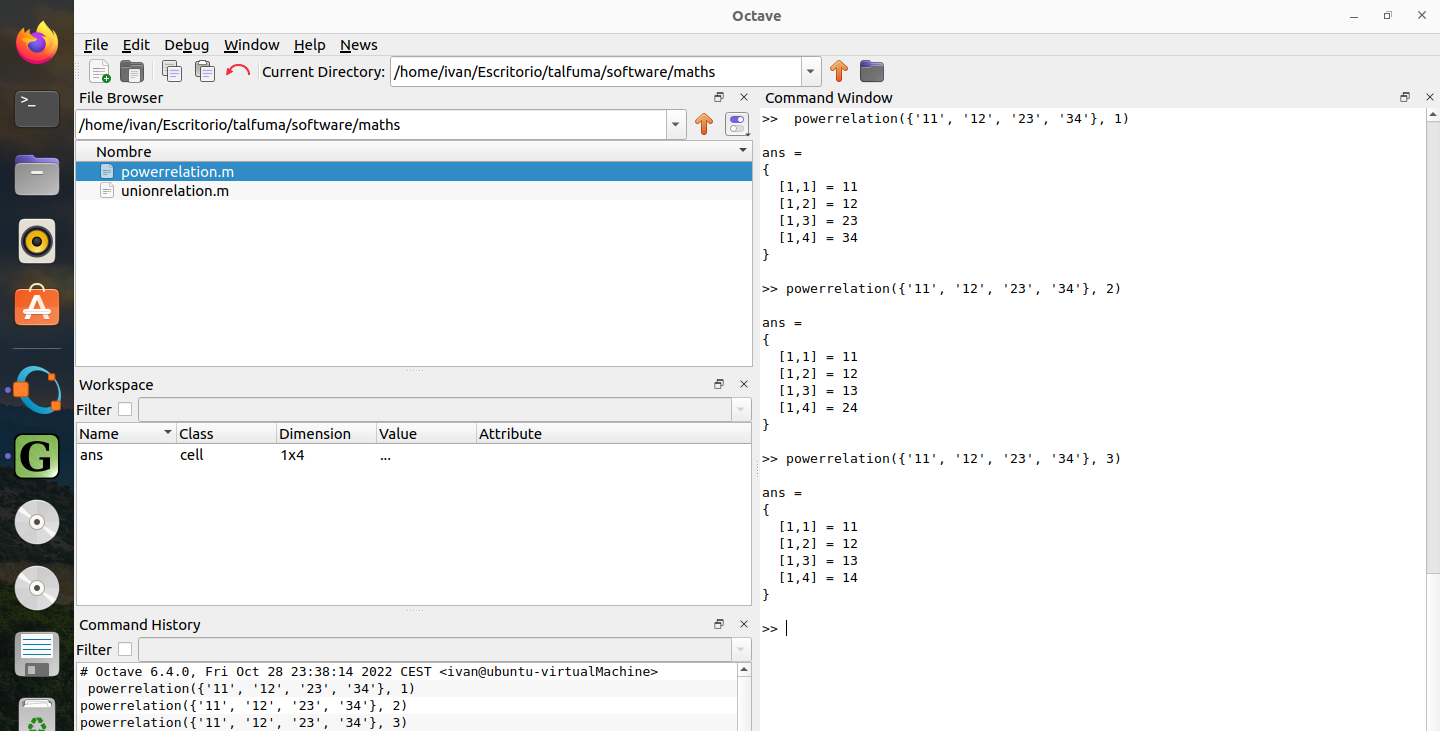
\includegraphics[width=1.1\linewidth]{Ejercicio1.png}
\end{document}